% !TEX root = ../thesis.tex
\chapter{一些重要的\LaTeX{}环境}\label{chap:evm}
\chapteren{Important \LaTeX{} environments}

\section{关于标签和引用}
\sectionen{About labels and references}

本模版中的公式、插图、表格和章节等,均用 \texttt{\char92 lable\{<key>\}}来在\LaTeX{}代码中标记位置,用 \texttt{\char92 ref\{<key>\}}来在代码中引用,其中 \texttt{<key>}为自定义的标签。为了避免混淆标签类型,建议将 \texttt{<key>} 命名为 \texttt{chap:key}、 \texttt{sec:key}、 \texttt{fig:key}、 \texttt{tab:key}、 \texttt{eqn:key} 等。本模版对 \texttt{hyperref} 中的标签名做了预设,已在引用中加上相应的前缀和后缀。\strong{在引用时,建议使用 \texttt{\char92 autoref\{<key>\}} 来引用,这样可以自动识别引用的类型。}例如,\autoref{chap:evm}是本章的引用,\autoref{sec:float}是第 \ref{chap:evm} 章的第 \ref{sec:float} 节的引用。

\section{关于浮动体}\label{sec:float}
\sectionen{About the floats}

在 \LaTeX{} 中,浮动体是一种用于排版图表( \texttt{figure} 和 \texttt{table} 等环境)和其他大块内容的机制。\LaTeX{} 会自动将浮动体放置在页面的合适位置,以保持最佳的页面排版效果。如果一个浮动体在当前页面无法完全容纳,\LaTeX{} 会自动将其移动到下一页,并确保它的标题跟随着移动。

然而,有时浮动体的自动排版可能会导致一些问题,比如浮动体不在预期位置、过多的浮动体堆积等。我们可以用一些选项来设置浮动体的位置: 
\begin{itemize}
    \item \texttt{h}:当前位置(here),尽可能在当前位置放置浮动体;
    \item \texttt{t}:页面顶部(top),在页面顶部放置浮动体;
    \item \texttt{b}:页面底部(bottom),在页面底部放置浮动体;
    \item \texttt{p}:单独一页(page),将浮动体放置在单独的一页,这个页面上只包含浮动体,而没有其他文本内容;
    \item \texttt{!}:可以强制 忽略 \LaTeX{} 的一些限制,从而增加浮动体被放置的可能性。
\end{itemize}
此外,也可以适当调整文本内容,以便更好地容纳浮动体。

\section{公式示例} 
\sectionen{Formula example}

文中的公式建议使用 \texttt{amsmath} 宏包的 \texttt{align} 环境,该环境在对多行公式对齐方面具有很大的优势,具体的讨论请看知乎用户\href{https://www.zhihu.com/people/bo-xue-duo-wen-63}{\strong{博闻多学}}的\href{https://www.zhihu.com/question/477805692/answer/2045084752}{\strong{回答}}。

下面进行公式示例。普通公式:
\begin{align}
    a+b=x.
\end{align}
带有积分和分隔的公式:
\begin{align}
   \int^{\infty}_{0} f(x)\dd{x}, \qquad \oint_{C} f(z)\dd {z}.
\end{align}
多行公式:
\begin{align}
    \left(1+x\right)^{\alpha} &= \sum^{\infty}_{n=0}\left(\begin{matrix} \alpha \\ n\end{matrix}\right)x^n \nonumber \\ 
    &= 1 + \alpha x + \frac{\alpha(\alpha-1)}{2!}x^2 + \cdots + \frac{\alpha(\alpha-1)\cdots(\alpha-n+1)}{n!} + \cdots
    \label{eqn:taylorseries}
\end{align}
这里注意,对不需要编号的行要取消公式编号,即要在该行公式的源代码后边使用 \texttt{\char92 nonumber}命令。

公式的引用示例:\autoref{eqn:taylorseries}为泰勒级数。

一些特殊符号的\LaTeX{}命令见 \href{https://mirrors.ustc.edu.cn/CTAN/info/symbols/comprehensive/symbols-a4.pdf}{The Great, Big List of LATEX Symbols}。

\section{插图示例}
\sectionen{Figure example}

文中插图的插图建议使用 \texttt{graphicx}宏包的 \texttt{figure}环境搭配 \\ \texttt{\char92 includegraphics}命令。例如:
\begin{figure}[htbp]
	\centering
	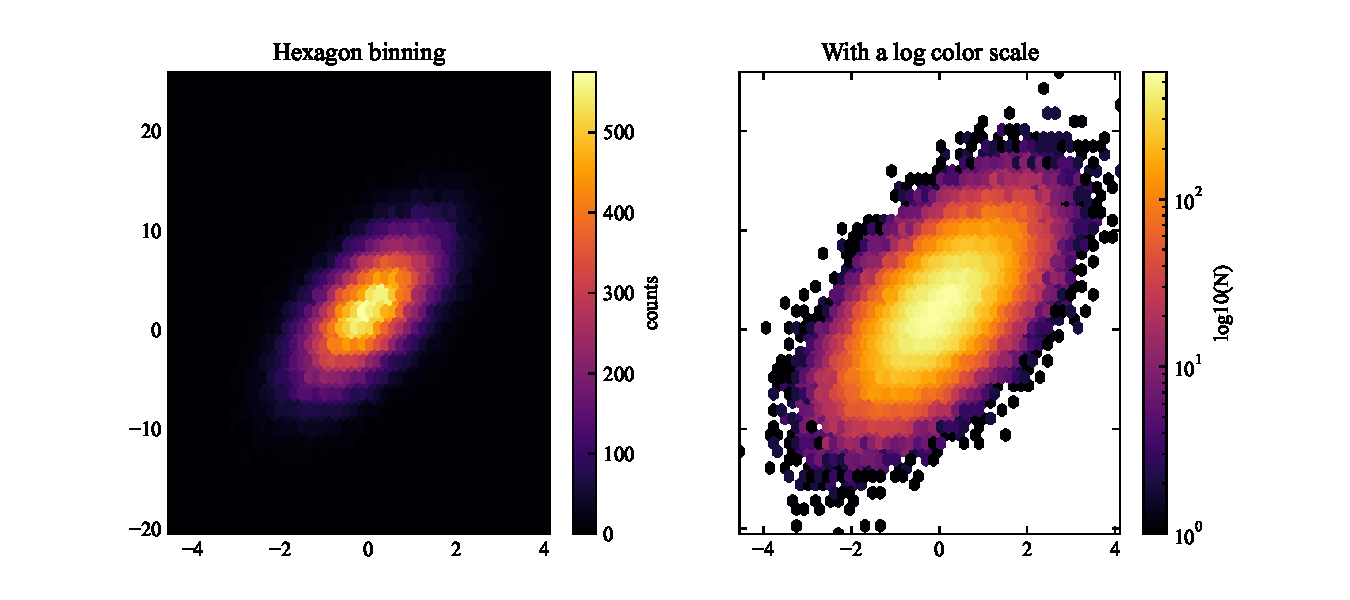
\includegraphics[width=1\textwidth]{figures/hexbin.pdf}
	\bicaption[六边形分bin图]{六边形分bin图六边形分bin图六边形分bin图六边形分bin图六边形分bin图六边形分bin图六边形分bin图六边形分bin图}[Hexagonal binned plot]
    {Hexagonal binned plot Hexagonal binned plot Hexagonal binned plot Hexagonal binned plot Hexagonal binned plot Hexagonal binned plot Hexagonal binned plot}
	\label{fig:hexbin}
\end{figure}
\begin{figure}[htbp]
	\centering
    \begin{subfigure}{0.45\textwidth}
        \centering
	    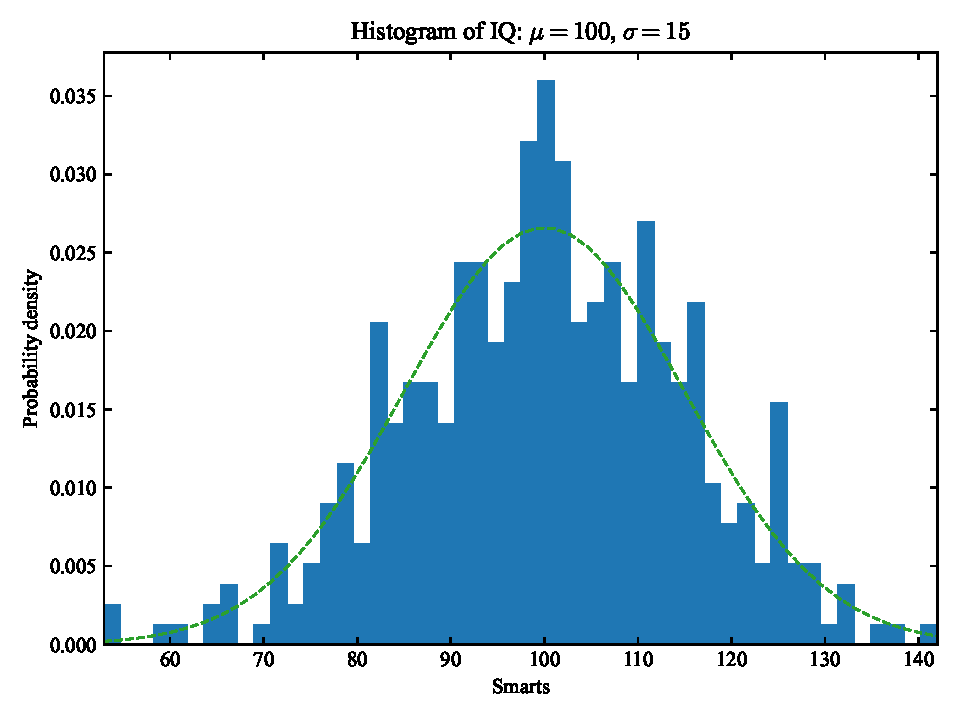
\includegraphics[width=1\textwidth]{figures/histogram.pdf}
	    \bicaption{柱状图}
        {Histogram}
    \end{subfigure}
    \begin{subfigure}{0.45\textwidth}
        \centering
	    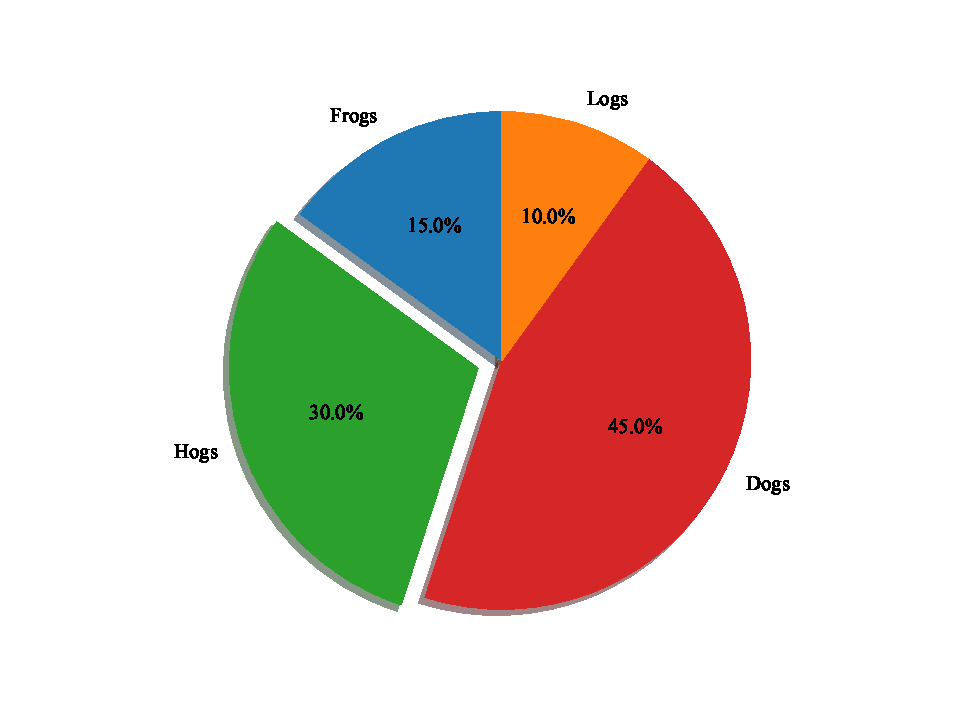
\includegraphics[width=1\textwidth]{figures/piechart.pdf}
	    \bicaption{饼状图}
        {Pie chart}
    \end{subfigure}
    \bicaption{子图示例}
    {Subfigure example}
    \label{fig:subfig}
\end{figure}

插图的引用示例:\autoref{fig:hexbin}是普通插图。

\section{表格示例}
\sectionen{Table example}

文中的表格建议使用 \texttt{table}环境里嵌套 \texttt{tabular}环境。
\begin{table}[htbp]
    \zihao{5}
    \bicaption{2022年北京冬奥会奖牌榜}
    {2022 Beijing winter Olympics medals}
    \label{tab:01}
    \centering
    \begin{tabular}{ccrrrr}
        \toprule
        总排名 & 国家/地区 & 金牌 & 银牌 & 铜牌 & 合计  \\ 
        \midrule
        1 & 挪威 & 16 & 8 & 13 & 37\\
        2 & 德国 & 12 & 10 & 5 & 27\\
        3 & 中国 & 9 & 4 & 2 & 15\\
        4 & 美国 & 8 & 10 & 7 & 25\\
        5 & 瑞典 & 8 & 5 & 5 & 18\\
        6 & 荷兰 & 8 & 5 & 4 & 17\\
        7 & 奥地利 & 7 & 7 & 4 & 18\\
        8 & 瑞士 & 7 & 2 & 5 & 14\\
        9 & 俄罗斯奥林匹克委员会\footnotemark & 6 & 12 & 14 & 32\\ 
        10 & 法国 & 5 & 7 & 2 & 14\\
        \bottomrule
    \end{tabular}
\end{table}
\footnotetext{俄罗斯由于被禁赛,不能以国家名义参加奥运会,不能使用国旗和国歌。因此俄罗斯代表团绕过禁令,以俄罗斯奥委会(Russian Olympic Committee)的名义参赛,以俄罗斯奥委会的会旗作为代表团的团旗,以柴可夫斯基的《第一钢琴协奏曲》作为团歌\cite{ROC}。}
这里需要注意,如果需要在表格内添加注释,请使用 \texttt{tablefootnote}宏包的 \texttt{\char92 tablefootnote}命令。如果要制作长表格,请使用 \texttt{longtable}宏包的 \texttt{longtable}环境,如\autoref{tab:longtable}。此外,本模版还对 \texttt{tabularray} 宏包进行了设置,可以使用 \texttt{longtblr} 环境来制作表格,如\autoref{tab:longtblr}和\autoref{tab:tblr}。\textbf{但注意:目前 \texttt{tabularray} 还未对双语标题和 List Of Tables 进行设置。}此外,在科技论文的排版中,一般使用三线表。推荐您使用 \texttt{booktabs} 宏包,该宏包支持三线表。本模版已经装载了 \texttt{booktabs} 宏包,可使用 \texttt{\char92 toprule}、 \texttt{\char92 midrule} 和 \texttt{\char92 bottomrule} 命令替换掉对应的 \texttt{\char92 hline} 即可。表格的引用示例:\autoref{tab:01}是2022年北京冬奥会奖牌榜。

{\zihao{5}%
\begin{longtable}[c]{ccc}
    \bicaption{长表格示例。\label{tab:longtable}}{Long Table Example.}\\
    
    \toprule
    Head & Head & Head \\
    \midrule
    \endfirsthead
    
    \multicolumn{3}{c}{\autoref{tab:longtable}(续)} \\
    \multicolumn{3}{c}{Table~\ref{tab:longtable}(Continued)} \\
    \toprule
    Head & Head & Head \\
    \midrule
    \endhead
    \bottomrule
    \multicolumn{3}{r}{下页续}
    
    \endfoot
    
    \bottomrule
    \endlastfoot
    
    Alpha & Beta & Gamma \\
    Epsilon & Zet & Eta \\
    Iota & Kappa & Lambda \\
    Nu & Xi & Omicron \\
    Rho & Sigma & Tau \\
    Phi & Chi & Psi \\
    Alpha & Beta & Gamma \\
    Epsilon & Zeta & Eta \\
    Iota & Kappa & Lambda \\
    Nu & Xi & Omicron \\
    Rho & Sigma & Tau \\
    Phi & Chi & Psi \\
    Alpha & Beta & Gamma \\
    Epsilon & Zeta & Eta \\
    Iota & Kappa & Lambda \\
    Nu & Xi & Omicron \\
    Rho & Sigma & Tau \\
    Phi & Chi & Psi \\
    Alpha & Beta & Gamma \\
    Epsilon & Zeta & Eta \\
    Iota & Kappa & Lambda \\
    Nu & Xi & Omicron \\
    Rho & Sigma & Tau \\
    Phi & Chi & Psi \\
    Alpha & Beta & Gamma \\
    Epsilon & Zeta & Eta \\
    Iota & Kappa & Lambda \\
    Nu & Xi & Omicron \\
    Rho & Sigma & Tau \\
    Phi & Chi & Psi \\
    Alpha & Beta & Gamma \\
    Epsilon & Zeta & Eta \\
    Iota & Kappa & Lambda \\
    Nu & Xi & Omicron \\
    Rho & Sigma & Tau \\
    Phi & Chi & Psi \\
    Foot & Foot & Foot \\
\end{longtable}
}
\begin{longtblr}[
    caption = {一个很长很长的表格示例。},
    entry = {长表格短标题},
    label = {tab:longtblr},
    note{$\dag$} = {It is a long long long long long long footnote.},
    remark{注意} = {Some general note. Some general note. Some general note.},
]{
    colspec = {XXX}, width = 0.85\linewidth,
    rowhead = 2, rowfoot = 0,
    % row{odd} = {sysugreen!50}, row{even} = {sysured!50},
    row{1-Z} = {font=\zihao{5}},
}
    \toprule
    Head & Head & Head \\
    \midrule
    Alpha & Beta & Gamma \\
    Epsilon & Zet & Eta \\
    Iota & Kappaa\TblrNote{$\dag$} & Lambda \\
    Nu & Xi & Omicron \\
    Rho & Sigma & Tau \\
    Phi & Chi & Psi \\
    Alpha & Beta & Gamma \\
    Epsilon & Zeta & Eta \\
    Iota & Kappa & Lambda \\
    Nu & Xi & Omicron \\
    Rho & Sigma & Tau \\
    Phi & Chi & Psi \\
    Alpha & Beta & Gamma \\
    Epsilon & Zeta & Eta \\
    Iota & Kappa & Lambda \\
    Nu & Xi & Omicron \\
    Rho & Sigma & Tau \\
    Phi & Chi & Psi \\
    Alpha & Beta & Gamma \\
    Epsilon & Zeta & Eta \\
    Iota & Kappa & Lambda \\
    Nu & Xi & Omicron \\
    Rho & Sigma & Tau \\
    Phi & Chi & Psi \\
    Alpha & Beta & Gamma \\
    Epsilon & Zeta & Eta \\
    Iota & Kappa & Lambda \\
    Nu & Xi & Omicron \\
    Rho & Sigma & Tau \\
    Phi & Chi & Psi \\
    Alpha & Beta & Gamma \\
    Epsilon & Zeta & Eta \\
    Iota & Kappa & Lambda \\
    Nu & Xi & Omicron \\
    Rho & Sigma & Tau \\
    Phi & Chi & Psi \\
    Foot & Foot & Foot \\
    \bottomrule
\end{longtblr}
\begin{talltblr}[
    caption = {一个正常表格示例。},
    entry = {正常表格短标题},
    label = {tab:tblr},
    note{$\dag$} = {It is a footnote.},
    remark{注意} = {Some general note. Some general note. Some general note.},
]{
    colspec = {XXX}, width = 0.85\linewidth,
    rowhead = 2, rowfoot = 0,
    row{1-Z} = {font=\zihao{5}},
}
    \toprule
    Head & Head & Head \\
    \midrule
    Alpha & Beta & Gamma \\
    Epsilon & Zet & Eta \\
    Iota & Kappa\TblrNote{$\dag$} & Lambda \\
    Nu & Xi & Omicron \\
    Rho & Sigma & Tau \\
    Phi & Chi & Psi \\
    Foot & Foot & Foot \\
    \bottomrule
\end{talltblr}

\section{其他数学环境示例}
\sectionen{Other theorem environments example}

以下是本模版预设的数学环境示例:

\begin{assumption}[连续统假设]
    不存在一个基数绝对大于可数集而绝对小于实数集的集合。
\end{assumption}
\begin{axiom}[平行公理]
    若两条直线都与第三条直线相交,并且在同一边的内角之和小于两个直角,则这两条直线在这一边必定相交。
\end{axiom}
\begin{conjecture}[黎曼猜想]
    黎曼$\zeta$函数
    \begin{align}
        \zeta(s) = \frac{1}{1^s} + \frac{1}{2^s} + \frac{1}{3^s} + \frac{1}{4^s} + \cdots
    \end{align}
    非平凡点的实数部分是$1/2$。
\end{conjecture}
\begin{definition}[定义的定义]
    对一个概念或者词或者词组的定义是描写其内涵,即描写其所有和仅有的元素的共有特征。其外延是所有这个概念、词或者词组包含的事物。
\end{definition}
\begin{example}
    举个栗子。
\end{example}
\begin{exercise}
    TiMi,发出学习的声音。
\end{exercise}
\begin{lemma}[欧几里得引理]
    如果一个正整数整除另外两个正整数的乘积,第一个整数与第二个整数互质,那么第一个整数整除第三个整数。
\end{lemma}
\begin{problem}
    花儿为什么这样红?
\end{problem}
\begin{proposition}
    通过一个不在直线上的点,有且仅有一条不与该直线相交的直线。
\end{proposition}
\begin{theorem}[诺特定理]
    对于每个局部作用下的可微对称性,存在一个对应的守恒流。另言之,每个连续对称性都有着相应的守恒定律。
\end{theorem}
\begin{corollary}
    推论往往在定理后出现。如果命题B能够被简单明了的从命题A推导出,则称B为A的推论。
\end{corollary}
\begin{solution}
    这个问题无解。
\end{solution}
\begin{proof}
    因为爱情,不会轻易悲伤,所以一切都是幸福的模样。
\end{proof}

\section{算法环境}

在论文中插入算法,我们使用的是 \texttt{algorithm2e} 宏包的 \texttt{algorithm} 环境。在 \texttt{algorithm} 环境中,你可以使用 \texttt{\char92 For}、 \texttt{\char92 While}、 \texttt{\char92 If}、 \texttt{\char92 eIF} 等命令来编写算法的结构,具体的使用方法请参考 \texttt{algorithm2e} 宏包的文档。例如\autoref{algo:algorithm} 和\autoref{algo:IR} 是算法示例。

\begin{algorithm}[htb]
    \caption{算法示例 \\ \textbf{Algorithm~\ref{algo:algorithm}:} How to write algorithms}
    \label{algo:algorithm}
    \SetAlgoLined
    \KwData{this text}
    \KwResult{how to write algorithm with \LaTeX2e }
    initialization\;
    \While{not at end of this document}{
      read current\;
      \eIf{understand}{
        go to next section\;
        current section becomes this one\;
        }{
        go back to the beginning of current section\;
        }
      }
\end{algorithm}
\begin{algorithm}[p]
    \DontPrintSemicolon
    \KwData{$G=(X,U)$ such that $G^{tc}$ is an order.}
    \KwResult{$G’=(X,V)$ with $V\subseteq U$ such that $G’^{tc}$ is an
    interval order.}
    \Begin{
    $V \longleftarrow U$\;
    $S \longleftarrow \emptyset$\;
    \For{$x\in X$}{
    $NbSuccInS(x) \longleftarrow 0$\;
    $NbPredInMin(x) \longleftarrow 0$\;
    $NbPredNotInMin(x) \longleftarrow |ImPred(x)|$\;
    }
    \For{$x \in X$}{
    \If{$NbPredInMin(x) = 0$ {\bf and} $NbPredNotInMin(x) = 0$}{
    $AppendToMin(x)$}
    }
    \nl\While{$S \neq \emptyset$}{\label{InRes1}
    \nlset{REM} remove $x$ from the list of $T$ of maximal index\;\label{InResR}
    \lnl{InRes2}\While{$|S \cap ImSucc(x)| \neq |S|$}{
    \For{$ y \in S-ImSucc(x)$}{
    \{ remove from $V$ all the arcs $zy$ : \}\;
    \For{$z \in ImPred(y) \cap Min$}{
    remove the arc $zy$ from $V$\;
    $NbSuccInS(z) \longleftarrow NbSuccInS(z) - 1$\;
    move $z$ in $T$ to the list preceding its present list\;
    \{i.e. If $z \in T[k]$, move $z$ from $T[k]$ to
    $T[k-1]$\}\;
    }
    $NbPredInMin(y) \longleftarrow 0$\;
    $NbPredNotInMin(y) \longleftarrow 0$\;
    $S \longleftarrow S - \{y\}$\;
    $AppendToMin(y)$\;
    }
    }
    $RemoveFromMin(x)$\;
    }
    }
    \caption{IntervalRestriction}
    \label{algo:IR}
\end{algorithm}

\section{代码示例}
\sectionen{Code listings example}

在论文中插入代码,我们使用的是 \texttt{listings}宏包的 \texttt{lstlisting}环境,如:
\begin{lstlisting}[language=Python,
    caption1=Python 画图代码1,
    caption2=Python ploting code 1]
import numpy as np
import matplotlib.pyplot as plt

# Fixing random state for reproducibility
np.random.seed(19680801)

dt = 0.01
t = np.arange(0, 30, dt)
nse1 = np.random.randn(len(t))                 # white noise 1
nse2 = np.random.randn(len(t))                 # white noise 2
    
# Two signals with a coherent part at 10Hz and a random part
s1 = np.sin(2 * np.pi * 10 * t) + nse1
s2 = np.sin(2 * np.pi * 10 * t) + nse2

fig, axs = plt.subplots(2, 1)
axs[0].plot(t, s1, t, s2)
axs[0].set_xlim(0, 2)
axs[0].set_xlabel('time')
axs[0].set_ylabel('s1 and s2')
axs[0].grid(True)
 
cxy, f = axs[1].cohere(s1, s2, 256, 1. / dt)
axs[1].set_ylabel('coherence')

fig.tight_layout()
plt.show()
\end{lstlisting}
或 \texttt{\char92 lstinputlisting}命令,如:
\lstinputlisting[language=Python,
    caption1=Python 画图代码2,
    caption2=Python ploting code 2,
    label=lst:cohere]
{codes/cohere.py}
代码可以使用 \texttt{caption} 选项,如果是双语标题请分别使用 \texttt{caption1} 和 \texttt{caption2}。例如\autoref{lst:cohere} 的\TeX{}源代码为:
\begin{lstlisting}[language=TeX]
\lstinputlisting[language=Python,
    caption1=Python 画图代码2,
    caption2=Python ploting code 2,
    label=lst:cohere]
{codes/cohere.py}
\end{lstlisting}

\section{参考文献}\label{sec:bibstyle}
\sectionen{References example}

\subsection{引用格式}
\subsectionen{Citation format}

\textbf{注意:本模版旧的参考文献引用格式已经弃用,转用国标,使用的是 Zeping Lee 等人开发的 \texttt{gbt7714} 宏包,具体的使用方法请参考 \url{https://github.com/zepinglee/gbt7714-bibtex-style}。}

\texttt{gbt7714} 宏包的引用标注方法与 \texttt{natbib} 宏包类似,分别有 \texttt{\char92 cite} 、\texttt{\char92 citep} 和 \texttt{\char92 citet} 三种命令,其中在顺序编码制(\texttt{numberical})中 \texttt{\char92 cite} 命令同 \texttt{\char92 citep},而在著者-出版年制(\texttt{author-year})中 \texttt{\char92 cite} 命令同 \texttt{\char92 citet}。引用有可选项,可以把引文页码放进来。此外,如果想用正文模式,还可以使用 \texttt{\char92 citestyle\{numbers\}} 命令(除非你想此后的引用标注都是正文模式,否则请用一对花括号将它的作用范围限制住,以防溢出,并且只在顺序编码制中使用)。例如:
\begin{enumerate}
    \item 这是一个期刊的引用\cite{LIGOScientific:2017zic};
    \item 这是一个加入作者的期刊引用:\citet{ZhaoWen:2017twxjz}在研究中发现……
    \item 这是一个图书的引用\cite{Rubakov:2017xzr};
    \item 这是一个加入引文页码的图书的引用\cite[92]{Zhang:2021};
    \item 这是一个研讨会论文的引用:文献{\citestyle{numbers}\cite{Tanikawa:2021+x}}中说明……
    \item 这是博士论文的引用\citep{Migenda:2019xbm,HuangGuoYuan:2020},这是硕论文的引用\citep{Shojaeifar:2015csv,SongRen:2020};
    \item 这是电子文献的引用\citep{Piro:2021oaa,bilibili:read}。
    \item 这是报纸的引用\citep{Li:2005}。
\end{enumerate}

\section{注释}
\sectionen{Remarks}

注释:可以用“脚注”或“文后注”来标注引用著作中的一些观点和案例,但全文标注方式应统一,本文统一使用“脚注”\footnote{这里是注释内容。}。注释个数不宜过多,一般不超过 10 个。